\documentclass{article}

% preamble
\def\npart{III}
\def\nyear{2023}
\def\nterm{Michaelmas}
\def\nlecturer{Prof Perla Sousi}
\def\ncourse{advanced Probability}
\def\draft{Incomplete}

\ifx \nauthor\undefined
  \def\nauthor{Ya\"el Dillies}
\else
\fi

\author{Based on lectures by \nlecturer \\\small Notes taken by \nauthor}
\date{\nterm\ \nyear}
\ifdefined\draft
\title{Part \npart\ -- \ncourse\ (\draft)}
\else
\title{Part \npart\ -- \ncourse}
\fi

\usepackage[utf8]{inputenc}
\usepackage{amsmath}
\usepackage{amsthm}
\usepackage{amssymb}
\usepackage{cancel}
\usepackage{enumerate}
\usepackage{mathtools}
\usepackage{fancyhdr}
\usepackage{graphicx}
\usepackage[dvipsnames]{xcolor}
\usepackage{tikz}
\usepackage{wrapfig}
\usepackage{centernot}
\usepackage{float}
\usepackage{braket}
\usepackage{marginnote}
\usepackage{mathdots}
\usepackage{mathrsfs}
\usepackage{ifthen}
\usepackage{imakeidx}
\usepackage{parskip}
\usepackage{relsize}
\usepackage{tabularx}
\usepackage[hypcap=true]{caption}
\usepackage[shortlabels]{enumitem}
\usepackage[pdftex,
  colorlinks=true,
  linkcolor=lblue,
  pdfauthor={\nauthor},
  pdfsubject={Cambridge Maths Notes: Part \npart\ - \ncourse},
  pdftitle={\ncourse - Part \npart},
pdfkeywords={Cambridge Mathematics Maths Math \npart\ \nterm\ \nyear\ \ncourse}]{hyperref}

\usepackage[capitalise,nameinlink,noabbrev]{cleveref}
\usepackage{nameref}
\usepackage[margin=1.5in,a4paper]{geometry}

\reversemarginpar
\newcommand{\lecnum}[1]{\leavevmode\marginnote{\emph{Lecture #1}}\ignorespaces}
\newcounter{lecturenumber}
\newcommand{\newlec}{\stepcounter{lecturenumber}\lecnum{\arabic{lecturenumber}}}

% Theorems
\theoremstyle{definition}
\newtheorem*{aim}{Aim}
\newtheorem*{assumption}{Assumption}
\newtheorem*{axiom}{Axiom}
\newtheorem*{claim}{Claim}
\newtheorem*{cor}{Corollary}
\newtheorem*{conjecture}{Conjecture}
\newtheorem*{defi}{Definition}
\newtheorem*{eg}{Example}
\newtheorem*{egs}{Examples}
\newtheorem*{ex}{Exercise}
\newtheorem*{fact}{Fact}
\newtheorem*{goal}{Goal}
\newtheorem*{idea}{Idea}
\newtheorem*{law}{Law}
\newtheorem*{lemma}{Lemma}
\newtheorem*{notation}{Notation}
\newtheorem*{note}{Note}
\newtheorem*{obs}{Observation}
\newtheorem*{prop}{Proposition}
\newtheorem*{properties}{Properties}
\newtheorem*{question}{Question}
\newtheorem*{rrule}{Rule}
\newtheorem*{steps}{Steps}
\newtheorem*{thm}{Theorem}

\newtheorem*{rmk}{Remark}
\newtheorem*{rmks}{Remarks}
\newtheorem*{warning}{Warning}
\newtheorem*{exercise}{Exercise}

\newtheorem{nthm}{Theorem}[section]
\newtheorem{ndef}[nthm]{Definition}
\newtheorem{nprop}[nthm]{Proposition}
\newtheorem{nconjecture}{Conjecture}
\newtheorem{ncor}[nthm]{Corollary}
\newtheorem{nex}[nthm]{Example}
\newtheorem{nlemma}[nthm]{Lemma}
\newtheorem{problem}[nthm]{Problem}

% Command redirections
\let\P\oldP
\let\oldemptyset\emptyset
\let\emptyset\varnothing

% Letter shorthands
\newcommand{\C}{\mathbb C}
\newcommand{\bbE}{\mathbb E}
\newcommand{\F}{\mathbb F}
\newcommand{\K}{\mathbb K}
\newcommand{\N}{\mathbb N}
\newcommand{\P}{\mathbb P}
\newcommand{\Q}{\mathbb Q}
\newcommand{\R}{\mathbb R}
\newcommand{\Z}{\mathbb Z}
\newcommand{\mcA}{\mathcal A}
\newcommand{\mcB}{\mathcal B}
\newcommand{\mcC}{\mathcal C}
\newcommand{\mcD}{\mathcal D}
\newcommand{\mcE}{\mathcal E}
\newcommand{\mcF}{\mathcal F}
\newcommand{\mcG}{\mathcal G}
\newcommand{\mcH}{\mathcal H}
\newcommand{\mcM}{\mathcal M}
\newcommand{\mcN}{\mathcal N}
\newcommand{\mcO}{\mathcal O}
\newcommand{\mcP}{\mathcal P}
\newcommand{\mcQ}{\mathcal Q}
\newcommand{\mcR}{\mathcal R}
\newcommand{\mcS}{\mathcal S}
\newcommand{\mcT}{\mathcal T}
\newcommand{\mcU}{\mathcal U}
\newcommand{\mcV}{\mathcal V}
\newcommand{\eps}{\varepsilon}
\newcommand{\Eps}{\mathcal E}

\newcommand{\curlybrack}[1]{\left\{ #1\right\}}
\newcommand{\abs}[1]{\left\lvert #1\right\rvert}
\newcommand{\norm}[1]{\left\lVert #1\right\rVert}
\newcommand{\inn}[2]{\left\langle #1, #2\right\rangle}
\newcommand{\floor}[1]{\left\lfloor #1\right\rfloor}
\newcommand{\ceil}[1]{\left\lceil #1\right\rceil}
\newcommand{\doublesqbrack}[1]{[\![#1]\!]}

\newcommand{\imp}{\implies}
\newcommand{\for}{\forall}
\newcommand{\mor}{\rightarrow}
\newcommand{\nin}{\notin}
\newcommand{\comp}{\circ}
\newcommand{\union}{\cup}
\newcommand{\inter}{\cap}
\newcommand{\Union}{\bigcup}
\newcommand{\Inter}{\bigcap}
\newcommand{\hatplus}{\mathbin{\widehat{+}}}
\newcommand{\symdif}{\mathbin\varbigtriangleup}
\newcommand{\aeeq}{\overset{\text{ae}}=}
\newcommand{\lexlt}{\overset{\text{lex}}<}
\newcommand{\colexlt}{\overset{\text{colex}}<}
\newcommand{\wtendsto}{\overset w\mor}
\newcommand{\wstartendsto}{\overset{w*}\mor}
\renewcommand{\vec}[1]{\boldsymbol{\mathbf{#1}}}
\renewcommand{\bar}[1]{\overline{#1}}

\newcommand*{\E}{
  \mathop{
    \mathchoice{\vcenter{\hbox{\larger[4]$\mathbb{E}$}}}
               {\kern0pt\mathbb{E}}
               {\kern0pt\mathbb{E}}
               {\kern0pt\mathbb{E}}
  }\displaylimits
}

\newcommand{\named}[1]{\textbf{#1}\index{#1}}
\newcommand{\bonusnamed}[1]{\textbf{#1}\index{#1@*#1}}

\let\Im\relax
\let\Re\relax

\DeclareMathOperator{\Ber}{Ber}
\DeclareMathOperator{\conv}{conv}
\DeclareMathOperator{\diam}{diam}
\DeclareMathOperator{\codim}{codim}
\DeclareMathOperator{\esssup}{ess sup}
\DeclareMathOperator{\Ext}{Ext}
\DeclareMathOperator{\id}{id}
\DeclareMathOperator{\im}{im}
\DeclareMathOperator{\Im}{Im}
\DeclareMathOperator{\interior}{int}
\DeclareMathOperator{\lhs}{LHS}
\DeclareMathOperator{\rank}{rank}
\DeclareMathOperator{\Re}{Re}
\DeclareMathOperator{\rhs}{RHS}
\DeclareMathOperator{\Span}{Span}
\DeclareMathOperator{\Spec}{Spec}
\DeclareMathOperator{\supp}{supp}
\DeclareMathOperator{\Var}{Var}

\definecolor{lblue}{rgb}{0., 0.05, 0.6}
\definecolor{mblue}{rgb}{0.2, 0.3, 0.8}
\definecolor{morange}{rgb}{1, 0.5, 0}
\definecolor{mgreen}{rgb}{0.1, 0.4, 0.2}
\definecolor{mred}{rgb}{0.5, 0, 0}

\colorlet{bred}{red}
\colorlet{bblue}{Cyan!50!blue}
\colorlet{byellow}{yellow}
\colorlet{bgreen}{YellowGreen!50!Green}
\colorlet{borange}{red!20!yellow}
\colorlet{bpurple}{violet}

\newcommand{\red}[1]{\textcolor{bred}{#1}}
\newcommand{\green}[1]{\textcolor{bgreen}{#1}}
\newcommand{\blue}[1]{\textcolor{bblue}{#1}}
\newcommand{\yellow}[1]{\textcolor{byellow}{#1}}
\newcommand{\orange}[1]{\textcolor{borange}{#1}}
\newcommand{\purple}[1]{\textcolor{bpurple}{#1}}

\pagestyle{fancy}
\fancyhf{}
\fancyfoot[R]{\href{yaeldillies.github.io/maths-notes}{\color{lblue}{Updated online}}}
\fancyfoot[C]{\thepage}
\ifdefined\draft
\fancyfoot[L]{\emph{\draft}}
\else
\fi
\renewcommand{\headrulewidth}{0pt}
\renewcommand{\footrulewidth}{0.2pt}

% Counters and table of content

\swapnumbers
\reversemarginpar

\usetikzlibrary{positioning, decorations.pathmorphing, decorations.text, calc, backgrounds, fadings}
\tikzset{node/.style = {circle,draw,inner sep=0.8mm}}

\makeindex[intoc]
\swapnumbers
\reversemarginpar

\usetikzlibrary{positioning, decorations.pathmorphing, decorations.text, calc, backgrounds, fadings}
\tikzset{node/.style = {circle,draw,inner sep=0.8mm}}

\makeindex[intoc]

\setcounter{section}{-1}

\newcommand{\brownian}[5]{% points, advance, rand factor, options, end label
\draw[#4] (0,0)
\foreach \x in {1,...,#1}
{   -- ++(#2,rand*#3)
}
node[right] {#5};
}

\pgfmathsetseed{23}

% and here we go!
\begin{document}
\maketitle

\tableofcontents

\clearpage

\section{Introduction}

\newlec

This course is concerned with advanced topics in modern probability theory. Two examples are

{\bf Martingales} \\
Martingales are processes indexed by discrete time such that
$$M_{n + 1} = M_n + \text{ extra randomness}$$
where
$$\E[\text{extra randomness} | M_n] = 0$$
A typical example is Markov chains.

{\bf Brownian motion} \\
Brownian motion is a continuous version of discrete random walks. It also arises naturally as the scaling limit of such. If $X_1, \dots$ are iid with mean $\mu$ and variance $\sigma^2$ and set $S_n = X_1 + \dots + X_n$, we have several theorems about
$$\frac{S_n}n \mor \mu$$
namely the Law of Large Numbers, the Central Limit Theorem, and Large Deviation results.

If we now set $B_t^{(n)} = \frac{S_{\floor{nt}} - \mu nt}{\sigma\sqrt n}$, we have that $B_t^{(n)}$ tends to Brownian motion as $n \mor \infty$.
\begin{figure}[h]
  \centering
  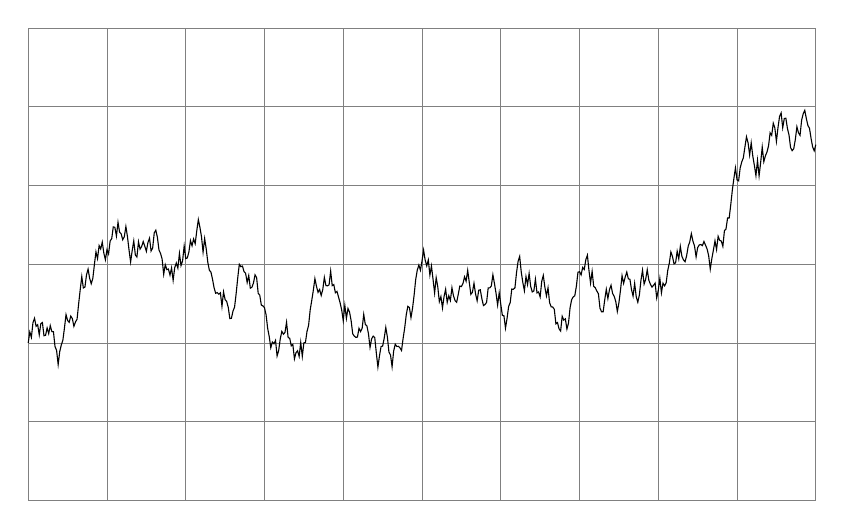
\begin{tikzpicture}
    \draw[help lines] (0,-2) grid (10,4);
    \brownian{500}{0.02}{0.2}{black}{}
  \end{tikzpicture}
  \caption{Standard Brownian motion}\label{fig:std-brown}
\end{figure}

TODO: Label Gaussian in figure

Recall {\bf Dirichlet's problem}: If $\mathcal D \subseteq \C$ is a simply connected domain and $f : \partial \mathcal D \mor \C$, can we find a harmonic function $u : \mathcal D \mor \C$ equal to $f$ on $\mathcal D$?

Brownian motion lets us define such a $u$ as follows: \\
Start a Brownian motion at $x \in \mathcal D$. Say it first hits the boundary of $\mathcal D$ in $B_T$. Evaluate $f$ at $B_T$. \\
Now take the expectation of the result and define
$$u(x) = \E[f(B_T)]$$
The resulting $u$ is harmonic and clearly equals $f$ on $\mathcal D$.

One can easily see that the corresponding construction in the discrete setting works by conditioning on the first move of the random walk.

TODO: Insert figure

\clearpage

\section{Conditional Expectation}

\subsection{Basic measure theory recap}

\begin{defi}
  A collection $\mathcal F$ of sets in $\Omega$ is a {\bf $\sigma$-algebra} if
  \begin{itemize}
    \item $\empty \in \mathcal F$
    \item If $A \in \mathcal F$, then $A^c \in \mathcal F$
    \item If $A_n \in \mathcal F$, then $\bigcup_n \in \mathcal F$
  \end{itemize}
\end{defi}

\begin{defi}
  $\P : \mathcal P(\mathcal P(\Omega))$ is a {\bf probability measure} if
  \begin{itemize}
    \item $\P(\empty) = 0$
    \item $\P(\Omega) = 1$
    \item When the $A_n$ are disjoint, $\P\left(\bigcup_n\right) = \sum_n \P(A_n)$
  \end{itemize}
\end{defi}

From now on, $\Omega$ will be a set equipped with a $\sigma$-algebra $\mathcal F$ and a probability measure $\P$.

\begin{defi}
  For $\mathcal A \subseteq \mathcal P(\Omega)$, define
  $$\sigma(\mathcal A) = \bigcap \{\mathcal F | \mathcal F \subseteq A \text{ is a $\sigma$-algebra}\}$$
  the smallest $\sigma$-algebra containing $\mathcal A$, aka {\bf $\sigma$-algebra generated by $\mathcal A$}. \\
  The {\bf Borel $\sigma$-algebra} $\mathcal B$ is the $\sigma$-algebra generated by the open sets in $\R$.
\end{defi}

\begin{defi}
  $X : \Omega \mor \R$ is a {\bf random variable} if $X$ is measurable with respect to $\mathcal B$, namely if $X^{-1}(U) \in \mathcal F$ for all opens $U \subseteq \R$.
\end{defi}

If the $X_i$, $i \in I$ are functions $\Omega \mor \R$, we write $\sigma(X_i | i \in I)$ for $\sigma(\{X_i^{-1}(U) | i \in I, U \subseteq \R \text{ open}\})$, the smallest $\sigma$-algebra making all the $X_i$ measurable.

\subsection{Expectiation}

\begin{defi}
  A {\bf simple function} is a function that can be written as a weighted sum of finitely many indicator functions.
\end{defi}

\begin{defi}
  For a simple function $f = \sum_i a_i 1_{A_i}$, we define
  $$\E[f] = \sum_i a_i \P(A_i)$$
  For a nonnegative function $f$, we define
  $$\E[f] = \sup_{g \le f \text{ simple}} \E[g]$$
  For an arbitrary function $f$, write $f = f^+ - f^-$ with $f^+, f^- \ge 0$, and define
  $$\E[f] = \E[f^+] - \E[f^-]$$
  assuming at least one of $\E[f^+], \E[f^-]$ is finite.
\end{defi}

\begin{defi}[Expectation conditional to an event]
  For $A \in \mathcal F$, define
  $$\E[X|A] = \frac{\E[1_A X]}{\P(A)}$$
\end{defi}

\newlec

\printindex
\end{document}